\documentclass[]{book}
\usepackage{lmodern}
\usepackage{amssymb,amsmath}
\usepackage{ifxetex,ifluatex}
\usepackage{fixltx2e} % provides \textsubscript
\ifnum 0\ifxetex 1\fi\ifluatex 1\fi=0 % if pdftex
  \usepackage[T1]{fontenc}
  \usepackage[utf8]{inputenc}
\else % if luatex or xelatex
  \ifxetex
    \usepackage{mathspec}
  \else
    \usepackage{fontspec}
  \fi
  \defaultfontfeatures{Ligatures=TeX,Scale=MatchLowercase}
\fi
% use upquote if available, for straight quotes in verbatim environments
\IfFileExists{upquote.sty}{\usepackage{upquote}}{}
% use microtype if available
\IfFileExists{microtype.sty}{%
\usepackage{microtype}
\UseMicrotypeSet[protrusion]{basicmath} % disable protrusion for tt fonts
}{}
\usepackage[margin=1in]{geometry}
\usepackage{hyperref}
\hypersetup{unicode=true,
            pdftitle={Practicos de Bioestadística 2},
            pdfauthor={Derek Corcoran},
            pdfborder={0 0 0},
            breaklinks=true}
\urlstyle{same}  % don't use monospace font for urls
\usepackage{natbib}
\bibliographystyle{apalike}
\usepackage{color}
\usepackage{fancyvrb}
\newcommand{\VerbBar}{|}
\newcommand{\VERB}{\Verb[commandchars=\\\{\}]}
\DefineVerbatimEnvironment{Highlighting}{Verbatim}{commandchars=\\\{\}}
% Add ',fontsize=\small' for more characters per line
\usepackage{framed}
\definecolor{shadecolor}{RGB}{248,248,248}
\newenvironment{Shaded}{\begin{snugshade}}{\end{snugshade}}
\newcommand{\AlertTok}[1]{\textcolor[rgb]{0.94,0.16,0.16}{#1}}
\newcommand{\AnnotationTok}[1]{\textcolor[rgb]{0.56,0.35,0.01}{\textbf{\textit{#1}}}}
\newcommand{\AttributeTok}[1]{\textcolor[rgb]{0.77,0.63,0.00}{#1}}
\newcommand{\BaseNTok}[1]{\textcolor[rgb]{0.00,0.00,0.81}{#1}}
\newcommand{\BuiltInTok}[1]{#1}
\newcommand{\CharTok}[1]{\textcolor[rgb]{0.31,0.60,0.02}{#1}}
\newcommand{\CommentTok}[1]{\textcolor[rgb]{0.56,0.35,0.01}{\textit{#1}}}
\newcommand{\CommentVarTok}[1]{\textcolor[rgb]{0.56,0.35,0.01}{\textbf{\textit{#1}}}}
\newcommand{\ConstantTok}[1]{\textcolor[rgb]{0.00,0.00,0.00}{#1}}
\newcommand{\ControlFlowTok}[1]{\textcolor[rgb]{0.13,0.29,0.53}{\textbf{#1}}}
\newcommand{\DataTypeTok}[1]{\textcolor[rgb]{0.13,0.29,0.53}{#1}}
\newcommand{\DecValTok}[1]{\textcolor[rgb]{0.00,0.00,0.81}{#1}}
\newcommand{\DocumentationTok}[1]{\textcolor[rgb]{0.56,0.35,0.01}{\textbf{\textit{#1}}}}
\newcommand{\ErrorTok}[1]{\textcolor[rgb]{0.64,0.00,0.00}{\textbf{#1}}}
\newcommand{\ExtensionTok}[1]{#1}
\newcommand{\FloatTok}[1]{\textcolor[rgb]{0.00,0.00,0.81}{#1}}
\newcommand{\FunctionTok}[1]{\textcolor[rgb]{0.00,0.00,0.00}{#1}}
\newcommand{\ImportTok}[1]{#1}
\newcommand{\InformationTok}[1]{\textcolor[rgb]{0.56,0.35,0.01}{\textbf{\textit{#1}}}}
\newcommand{\KeywordTok}[1]{\textcolor[rgb]{0.13,0.29,0.53}{\textbf{#1}}}
\newcommand{\NormalTok}[1]{#1}
\newcommand{\OperatorTok}[1]{\textcolor[rgb]{0.81,0.36,0.00}{\textbf{#1}}}
\newcommand{\OtherTok}[1]{\textcolor[rgb]{0.56,0.35,0.01}{#1}}
\newcommand{\PreprocessorTok}[1]{\textcolor[rgb]{0.56,0.35,0.01}{\textit{#1}}}
\newcommand{\RegionMarkerTok}[1]{#1}
\newcommand{\SpecialCharTok}[1]{\textcolor[rgb]{0.00,0.00,0.00}{#1}}
\newcommand{\SpecialStringTok}[1]{\textcolor[rgb]{0.31,0.60,0.02}{#1}}
\newcommand{\StringTok}[1]{\textcolor[rgb]{0.31,0.60,0.02}{#1}}
\newcommand{\VariableTok}[1]{\textcolor[rgb]{0.00,0.00,0.00}{#1}}
\newcommand{\VerbatimStringTok}[1]{\textcolor[rgb]{0.31,0.60,0.02}{#1}}
\newcommand{\WarningTok}[1]{\textcolor[rgb]{0.56,0.35,0.01}{\textbf{\textit{#1}}}}
\usepackage{longtable,booktabs}
\usepackage{graphicx,grffile}
\makeatletter
\def\maxwidth{\ifdim\Gin@nat@width>\linewidth\linewidth\else\Gin@nat@width\fi}
\def\maxheight{\ifdim\Gin@nat@height>\textheight\textheight\else\Gin@nat@height\fi}
\makeatother
% Scale images if necessary, so that they will not overflow the page
% margins by default, and it is still possible to overwrite the defaults
% using explicit options in \includegraphics[width, height, ...]{}
\setkeys{Gin}{width=\maxwidth,height=\maxheight,keepaspectratio}
\IfFileExists{parskip.sty}{%
\usepackage{parskip}
}{% else
\setlength{\parindent}{0pt}
\setlength{\parskip}{6pt plus 2pt minus 1pt}
}
\setlength{\emergencystretch}{3em}  % prevent overfull lines
\providecommand{\tightlist}{%
  \setlength{\itemsep}{0pt}\setlength{\parskip}{0pt}}
\setcounter{secnumdepth}{5}
% Redefines (sub)paragraphs to behave more like sections
\ifx\paragraph\undefined\else
\let\oldparagraph\paragraph
\renewcommand{\paragraph}[1]{\oldparagraph{#1}\mbox{}}
\fi
\ifx\subparagraph\undefined\else
\let\oldsubparagraph\subparagraph
\renewcommand{\subparagraph}[1]{\oldsubparagraph{#1}\mbox{}}
\fi

%%% Use protect on footnotes to avoid problems with footnotes in titles
\let\rmarkdownfootnote\footnote%
\def\footnote{\protect\rmarkdownfootnote}

%%% Change title format to be more compact
\usepackage{titling}

% Create subtitle command for use in maketitle
\newcommand{\subtitle}[1]{
  \posttitle{
    \begin{center}\large#1\end{center}
    }
}

\setlength{\droptitle}{-2em}

  \title{Practicos de Bioestadística 2}
    \pretitle{\vspace{\droptitle}\centering\huge}
  \posttitle{\par}
    \author{Derek Corcoran}
    \preauthor{\centering\large\emph}
  \postauthor{\par}
      \predate{\centering\large\emph}
  \postdate{\par}
    \date{2019-03-11}

\usepackage{booktabs}

\begin{document}
\maketitle

{
\setcounter{tocdepth}{1}
\tableofcontents
}
\hypertarget{requerimientos}{%
\chapter*{Requerimientos}\label{requerimientos}}
\addcontentsline{toc}{chapter}{Requerimientos}

Para comenzar el trabajo se necesita la última versión de R y RStudio \citep{R-base}.También se requiere de los paquetes \emph{pacman}, \emph{rmarkdown}, \emph{tidyverse} y \emph{tinytex}. Si no se ha usado R o RStudio anteriormente, el siguiente video muestra cómo instalar ambos programas y los paquetes necesarios para este curso en el siguiente \href{https://youtu.be/RtkCAKXsVbw}{link}.

El código para la instalación de esos paquetes es el siguiente:

\begin{Shaded}
\begin{Highlighting}[]
\KeywordTok{install.packages}\NormalTok{(}\StringTok{"pacman"}\NormalTok{, }\StringTok{"rmarkdown"}\NormalTok{, }\StringTok{"tidyverse"}\NormalTok{, }\StringTok{"tinytex"}\NormalTok{)}
\end{Highlighting}
\end{Shaded}

En caso de necesitar ayuda para la instalación, contactarse con el instructor del curso.

\hypertarget{antes-de-comenzar}{%
\section{Antes de comenzar}\label{antes-de-comenzar}}

Si nunca se ha trabajado con \texttt{R} antes de este curso, una buena herramienta es provista por el paquete \href{http://swirlstats.com/students.html}{Swirl} \citep{Kross2017}. Si deseas estar más preparado para el curso, realiza los primeros 7 módulos del programa \emph{R Programming: The basics of programming in R} que incluye:

\begin{itemize}
\tightlist
\item
  Basic Building Blocks
\item
  Workspace and Files
\item
  Sequences of Numbers
\item
  Vectors
\item
  Missing Values
\item
  Subsetting Vectors
\item
  Matrices and Data Frames
\end{itemize}

El siguiente link muestra un video explicativo de cómo usar el paquete swirl \href{https://youtu.be/w6L7Ye18yPE}{Video}

\hypertarget{descripcion-del-practico}{%
\section{Descripción del práctico}\label{descripcion-del-practico}}

Los prácticos de este curso se enfocan en aprender a realizar de manera práctica los conceptos enseñados en el cuso, pero además, usando herramientas interactivas y/o programáticas, el profundizar el entendimiento de ciertos conceptos teóricos y filosóficos del curso.

\hypertarget{objetivos-del-practico}{%
\section{Objetivos del práctico}\label{objetivos-del-practico}}

\begin{enumerate}
\def\labelenumi{\arabic{enumi}.}
\item
  Aprender el uso de R como ambiente estadístico de limpieza, exploración, visualización de datos.
\item
  Conocer y aplicar de manera aplicada los conceptos enseñados en el curso de Bioestadística 2.
\item
  Aprender buenas prácticas de recolección y estandarización de bases de datos, con la finalidad de optimizar el análisis de datos y la revisión de éstas por pares.
\item
  Realizar análisis críticos de la naturaleza de los datos al realizar análisis exploratorios, que permitirán determinar la mejor forma de comprobar hipótesis asociadas a estas bases de datos.
\end{enumerate}

\hypertarget{contenidos}{%
\section{Contenidos}\label{contenidos}}

\begin{itemize}
\item
  Capítulo \ref{Explorando} \emph{Análisis exploratorio y el primer ANOVA}: En este capítulo se aprenderá a cómo explorar, resumir y visualizar una base de datos utilizando el paquete tidyverse \citep{WickhamTidy2017}, además se realizarán un análisis básico de ANOVA
\item
  Capítulo \ref{Supuestos} \emph{Supuestos de ANOVA y mínimos cuadrados}
\item
  Capítulo \ref{Poder} \emph{Análisis de poder y primera tarea}
\item
  Capítulo \ref{Refs} \emph{Referencias}
\item
  Capítulo \ref{t-student} \emph{T de student}
\end{itemize}

\hypertarget{metodologia}{%
\section{Metodología}\label{metodologia}}

Clases prácticas donde cada estudiante trabajará con datos entregados para desarrollar análisis de datos. Además, se deberán generar informes, en base al trabajo con sus datos.

\hypertarget{evaluacion}{%
\section{Evaluación}\label{evaluacion}}

\begin{itemize}
\tightlist
\item
  Evaluación 1: Informe exploratorio de base de datos 25\%
\item
  Evaluación 2: Presentación 25\%
\item
  Evaluación 3: Informe final 50\%
\end{itemize}

\hypertarget{presentacion-de-introduccion}{%
\section{Presentación de introducción}\label{presentacion-de-introduccion}}

Para la introducción de los prácticos seguiremos un a presentación que se encuentra en este \href{http://www.derek-corcoran-barrios.com/AyudantiaStatsPres/Clase1/Clase1.html}{link}

\hypertarget{libros-de-consulta}{%
\section{Libros de consulta}\label{libros-de-consulta}}

Los principios de este curso están explicados en los siguientes libros gratuitos.

\begin{itemize}
\tightlist
\item
  Gandrud, Christopher. Reproducible Research with R and R Studio. CRC Press, 2013. Available for free in the following
  \href{https://englianhu.files.wordpress.com/2016/01/reproducible-research-with-r-and-studio-2nd-edition.pdf}{link}
\item
  Stodden, Victoria, Friedrich Leisch, and Roger D. Peng, eds. Implementing reproducible research. CRC Press, 2014. Available for free in the following \href{http://web.stanford.edu/~vcs/papers/ijclp-STODDEN-2009.pdf}{link}
\end{itemize}

\hypertarget{Explorando}{%
\chapter{Exploración de datos y tu primer ANOVA}\label{Explorando}}

\hypertarget{actividad-1-educacion-en-chile}{%
\section{Actividad 1 Educación en Chile}\label{actividad-1-educacion-en-chile}}

En esta actividad exploraremos los resultados de la PSU en Chile para el año 2017. Pueden encontrar la base de datos original en \href{https://es.datachile.io/geo/chile\#education}{Data Chile}.

Trataremos de determinar, usando el puntaje de la PSU como medida, si existen brechas en la educación chilena por tipo de institución. Para ello, primero trabajaremos realizando análisis exploratorios en base a gráficos y tablas resumen usando funciones del paquete \emph{tidyverse} \citep{WickhamTidy2017} en R.

La base de datos \emph{EducacionChile.csv} se encuentra disponible en webcursos o en \url{https://es.datachile.io/geo/chile\#education}.

\hypertarget{tablas-resumen-de-los-datos}{%
\subsection{Tablas resumen de los datos:}\label{tablas-resumen-de-los-datos}}

Lo primero que deben hacer es generar una tabla resumen usando el \emph{tidyverse} usando las funciones \emph{group\_by} para agrupar por variables y \emph{summarize} para resumir los datos, dentro de summarize podemos usar variables como:

\begin{itemize}
\tightlist
\item
  \textbf{mean()} promedio
\item
  \textbf{sd()} desviación estándar
\item
  \textbf{n()} número de muestras
\end{itemize}

a modo de ejemplo vemos la tabla \ref{tab:MediaIris} mostrando la media y número de muestras con la base de datos iris:

\begin{Shaded}
\begin{Highlighting}[]
\KeywordTok{data}\NormalTok{(}\StringTok{"iris"}\NormalTok{)}
\NormalTok{Table <-}\StringTok{ }\KeywordTok{group_by}\NormalTok{(iris, Species) }\OperatorTok\StringTok{ }\KeywordTok{summarize}\NormalTok{(}\DataTypeTok{Promedio =} \KeywordTok{mean}\NormalTok{(Petal.Length), }\DataTypeTok{N =} \KeywordTok{n}\NormalTok{())}
\end{Highlighting}
\end{Shaded}

\begin{Shaded}
\begin{Highlighting}[]
\NormalTok{knitr}\OperatorTok{::}\KeywordTok{kable}\NormalTok{(Table)}
\end{Highlighting}
\end{Shaded}

\begin{table}

\caption{\label{tab:MediaIris}Resumen con la media y número de muestras del largo de pétalo de las flores de tres especies del género Iris}
\centering
\begin{tabular}[t]{lrr}
\toprule
Species & Promedio & N\\
\midrule
setosa & 1.462 & 50\\
versicolor & 4.260 & 50\\
virginica & 5.552 & 50\\
\bottomrule
\end{tabular}
\end{table}

Basado en el resumen ¿Qué podemos decir de estos datos de educación en Chile?

\hypertarget{visualizacion-de-datos-con-ggplot2-tidyverse}{%
\subsection{Visualización de datos con ggplot2 (tidyverse)}\label{visualizacion-de-datos-con-ggplot2-tidyverse}}

El paquete \emph{ggplot2} \citep{WickhamGG2016} es una poderosa herramienta para graficar datos. Si desean ahondar en el uso de este paquete, pueden ver el siguiente link \url{http://zevross.com/blog/2014/08/04/beautiful-plotting-in-r-a-ggplot2-cheatsheet-3/}. En este caso, aprenderemos a graficar \emph{boxplots} y \emph{jitterplots}, dos opciones para visualizar una variable categórica versus una cuantitativa.

\hypertarget{uso-del-ggplot2}{%
\subsubsection{Uso del ggplot2}\label{uso-del-ggplot2}}

Su función principal es \emph{ggplot}, luego de cada función usaremos el símbolo \textbf{+} como usábamos el pipeline (\%\textgreater{}\%).

Primero usamos la función ggplot para determinar la base de datos y variables, acá las variables siempre van dentro de la función aes

\begin{Shaded}
\begin{Highlighting}[]
\KeywordTok{ggplot}\NormalTok{(MiBaseDeDatos, }\KeywordTok{aes}\NormalTok{(}\DataTypeTok{x =}\NormalTok{ VariableX, }\DataTypeTok{y =}\NormalTok{ VariableY)) }
\end{Highlighting}
\end{Shaded}

Luego agregamos el tipo de gráfico que queremos para nuestra figura usando el \textbf{+} como pipeline

\begin{Shaded}
\begin{Highlighting}[]
\KeywordTok{ggplot}\NormalTok{(MiBaseDeDatos, }\KeywordTok{aes}\NormalTok{(}\DataTypeTok{x =}\NormalTok{ VariableX, }\DataTypeTok{y =}\NormalTok{ VariableY)) }\OperatorTok{+}\StringTok{ }\KeywordTok{geom_boxplot}\NormalTok{()}
\end{Highlighting}
\end{Shaded}

\hypertarget{ejemplo-usando-la-base-de-datos-iris}{%
\subsubsection{Ejemplo usando la base de datos iris}\label{ejemplo-usando-la-base-de-datos-iris}}

\hypertarget{boxplot}{%
\paragraph{Boxplot}\label{boxplot}}

El siguiente código muestra como graficar un boxplot para la base de datos iris, la cual esta en R. En este caso graficaremos el largo del pétalo para cada especie (Figura \ref{fig:BoxplotIris}).

\begin{Shaded}
\begin{Highlighting}[]
\KeywordTok{data}\NormalTok{(}\StringTok{"iris"}\NormalTok{)}
\KeywordTok{ggplot}\NormalTok{(iris, }\KeywordTok{aes}\NormalTok{(}\DataTypeTok{x =}\NormalTok{ Species, }\DataTypeTok{y =}\NormalTok{ Petal.Length)) }\OperatorTok{+}\StringTok{ }\KeywordTok{geom_boxplot}\NormalTok{()}
\end{Highlighting}
\end{Shaded}

\begin{figure}
\centering
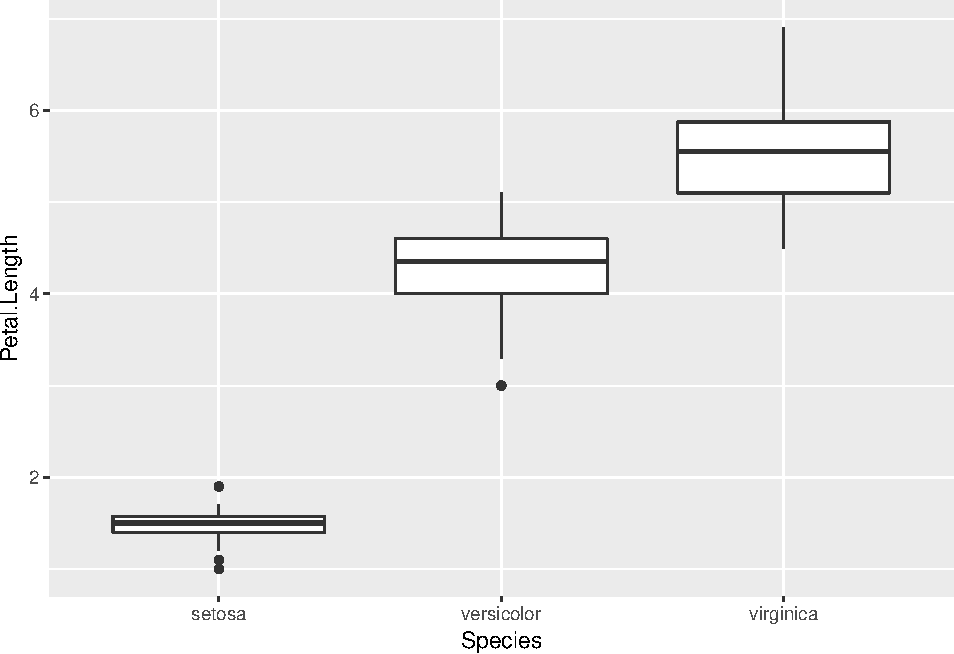
\includegraphics{AyduantiaStats_files/figure-latex/BoxplotIris-1.pdf}
\caption{\label{fig:BoxplotIris}Box plot del largo de petalo de tres especies del género Iris}
\end{figure}

En los Box Plots tenemos 4 visualizaciones:

\begin{itemize}
\tightlist
\item
  Mediana (linea gruesa)
\item
  Caja (Cuantiles 25\% y 75\%)
\item
  Bigotes (intervalo de confianza del 95\%)
\item
  Puntos Outlayers
\end{itemize}

Realice un boxplot de los datos de la educación de Chile, ¿Qué nos dice esto de los datos?

\hypertarget{jitter-plot}{%
\paragraph{Jitter plot}\label{jitter-plot}}

El jitter plot suma un punto por cada observación, lo cual nos permite entender un poco más la naturaleza de los datos. En general se le agrega a un box plot para tener mayor claridad en los datos (Figura \ref{fig:JitterIris}).

\begin{Shaded}
\begin{Highlighting}[]
\KeywordTok{data}\NormalTok{(}\StringTok{"iris"}\NormalTok{)}
\KeywordTok{ggplot}\NormalTok{(iris, }\KeywordTok{aes}\NormalTok{(}\DataTypeTok{x =}\NormalTok{ Species, }\DataTypeTok{y =}\NormalTok{ Petal.Length)) }\OperatorTok{+}\StringTok{ }\KeywordTok{geom_boxplot}\NormalTok{() }\OperatorTok{+}\StringTok{ }\KeywordTok{geom_jitter}\NormalTok{(}\KeywordTok{aes}\NormalTok{(}\DataTypeTok{color =}\NormalTok{ Species))}
\end{Highlighting}
\end{Shaded}

\begin{figure}
\centering
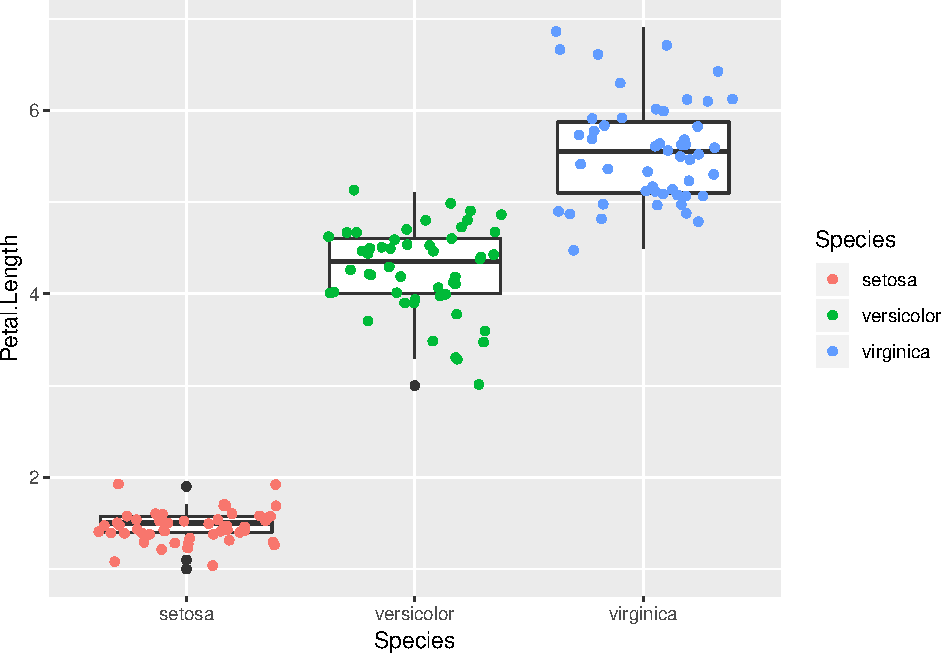
\includegraphics{AyduantiaStats_files/figure-latex/JitterIris-1.pdf}
\caption{\label{fig:JitterIris}Box plot y jitter plot juntos para el largo de petalo de tres especies del género Iris}
\end{figure}

\hypertarget{actividad-2-captacion-de-co2-en-plantas}{%
\section{Actividad 2 Captación de CO2 en plantas}\label{actividad-2-captacion-de-co2-en-plantas}}

Utilizaremos base de datos \(CO_2\) \citep{potvin1990statistical} enviada al curso. Esta base de datos, también presente en R, tiene las siguientes variables

\begin{itemize}
\tightlist
\item
  \textbf{Plant}: Identidad de cada planta
\item
  \textbf{Type}: Variedad de la planta (subespecie Quebec o Mississippi)
\item
  \textbf{Treatment}: Tratamiento de la planta, algunas fueron enfriadas la noche anterior (Chilled)
\item
  \textbf{conc}: Concentración ambiental de \(CO_2\)
\item
  \textbf{Uptake}: Captación de \(CO_2\) para cada planta en cada día
\end{itemize}

¿Hay diferencias entre la captación de \(CO_2\) en plantas tratadas y no tratadas?

\begin{itemize}
\tightlist
\item
  Genere tablas resumenes que le permitan explorar esta pregunta

  \begin{itemize}
  \tightlist
  \item
    ¿Existen variables que puedan confundir el resultado? ¿como trataría los datos para lidiar con esto?
  \end{itemize}
\item
  Genere gráficos exploratorios para contestar esta pregunta
\end{itemize}

\hypertarget{actividad-3-mi-primer-anova}{%
\section{Actividad 3 Mi primer ANOVA}\label{actividad-3-mi-primer-anova}}

En \emph{R} todos los modelos tienen la siguiente estructura \textbf{Funcion(y \textasciitilde{} x1 + x2 + \ldots{} + xn, data = MisDatos)}, donde la \textbf{Funcion} dice el modelo que queremos realizar (por ejemplo ANOVA, regresión lineal, modelos mixtos, etc.), \textbf{y} es la variable que queremos explicar, \textbf{x1} a \textbf{xn} son las variables explicativas, \textbf{\textasciitilde{}} es un símbolo que debe ser leído como explicado por y finalmente \textbf{data} es la base de datos que queremos utilizar, en un ANOVA (análisis de varianza), la función en cuestión es aov.

En el siguiente código vemos si el largo del pétalo de las flores del género \emph{Iris}, pueden ser explicados por la especie a la que estas plantas pertenecen, por lo que generamos un modelo llamado \emph{Primer.Anova} con la función \textbf{aov}.

\begin{Shaded}
\begin{Highlighting}[]
\NormalTok{Primer.Anova <-}\StringTok{ }\KeywordTok{aov}\NormalTok{(Petal.Length }\OperatorTok{~}\StringTok{ }\NormalTok{Species, }\DataTypeTok{data =}\NormalTok{ iris)}
\end{Highlighting}
\end{Shaded}

Para acceder a la tabla de resultados utilizamos la función \textbf{summary}

\begin{verbatim}
##              Df Sum Sq Mean Sq F value Pr(>F)    
## Species       2  437.1  218.55    1180 <2e-16 ***
## Residuals   147   27.2    0.19                   
## ---
## Signif. codes:  0 '***' 0.001 '**' 0.01 '*' 0.05 '.' 0.1 ' ' 1
\end{verbatim}

Si establecemos el valor de alfa en 0.05 y al ver en la tabla que el valor de p es menor a alfa, rechazamos la hipótesis nula de que las medias son iguales, y decidimos que la media del largo de pétalo es distinta entre las especies.

\hypertarget{ejercicio}{%
\subsection{Ejercicio}\label{ejercicio}}

Determine si para la base de datos \textbf{CO2} la captación de \(CO_2\) es distinto entre plantas con tratamiento de enfriamiento y sin enfriamiento.

\hypertarget{simulador-de-anova}{%
\subsection{Simulador de ANOVA}\label{simulador-de-anova}}

\href{http://admin.derek-corcoran-barrios.com/shiny/rstudio/sample-apps/Shiny2/}{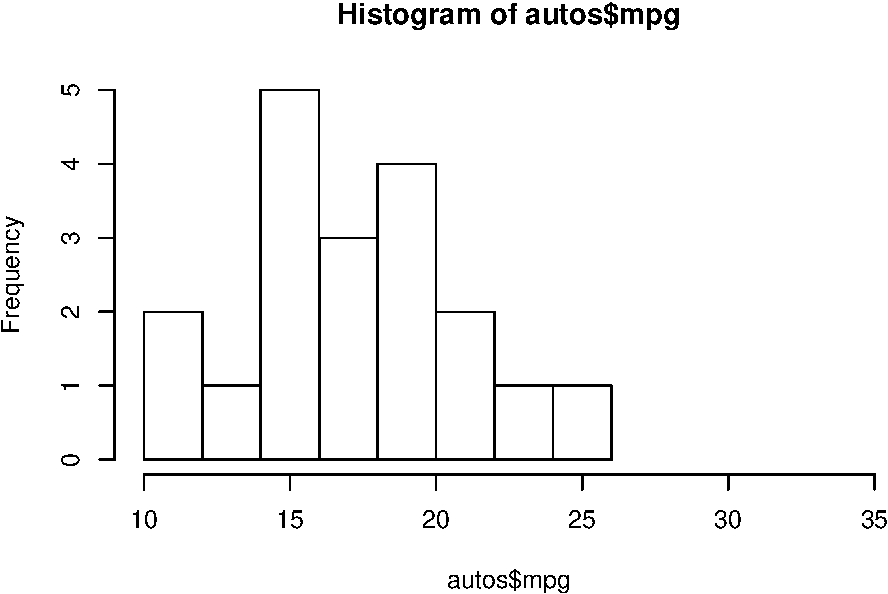
\includegraphics{AyduantiaStats_files/figure-latex/unnamed-chunk-10-1.pdf}}

\hypertarget{Supuestos}{%
\chapter{Supuestos de ANOVA y mínimos cuadrados}\label{Supuestos}}

\hypertarget{objetivos-de-este-practico}{%
\section{Objetivos de este práctico}\label{objetivos-de-este-practico}}

\begin{itemize}
\tightlist
\item
  Entender los supuestos de un ANOVA de una vía (independencia, aleatoriedad, homocedasticidad y normalidad)
\item
  Entender el concepto de mínimos cuadrados
\item
  Saber cuando realizar un ANOVA e interpretar sus resultados
\end{itemize}

\hypertarget{actividad-1-sueno-en-mamiferos}{%
\section{Actividad 1 Sueño en mamíferos}\label{actividad-1-sueno-en-mamiferos}}

En esta actividad intentaremos ver si hay diferencias en horas de sueño en mamíferos por Orden o dieta. Los datos fueron extraídos del trabajo de \citet{savage2007quantitative} y están incorporados en la base de datos de \emph{ggplot2} con el nombre de \emph{msleep}, pero estarán en webcursos en formato csv de todas formas. Para la guía los ejemplos se generarán en base a la base de datos \emph{InsectSprays} que está en \emph{R} y que fue extraída de \citet{beall1942transformation}, en la cual se testean la efectividad de insecticidas en Spray en la abundancia de insectos en plantaciones. Y en la base de datos \emph{iris} que ya fue entregada, en la que se miden distintas características florales de especies del genero \emph{Iris} \citep{anderson1935irises}.

\hypertarget{homogeneidad-de-varianza}{%
\subsection{Homogeneidad de varianza}\label{homogeneidad-de-varianza}}

\hypertarget{inspeccion-visual}{%
\subsubsection{Inspección visual}\label{inspeccion-visual}}

Lo primero que intentaremos explorar de forma visual y a partir de tests si es que hay homogeneidad de varianza, para esto usaremos boxplots, y jitter plots (Figura \ref{fig:Visual}), lo cual ya hemos hecho anteriormente:

\begin{Shaded}
\begin{Highlighting}[]
\KeywordTok{ggplot}\NormalTok{(InsectSprays, }\KeywordTok{aes}\NormalTok{(}\DataTypeTok{x =}\NormalTok{ spray, }\DataTypeTok{y =}\NormalTok{ count)) }\OperatorTok{+}\StringTok{ }\KeywordTok{geom_boxplot}\NormalTok{() }\OperatorTok{+}\StringTok{ }\KeywordTok{geom_jitter}\NormalTok{(}\KeywordTok{aes}\NormalTok{(}\DataTypeTok{color =}\NormalTok{ spray)) }
\end{Highlighting}
\end{Shaded}

\begin{figure}
\centering
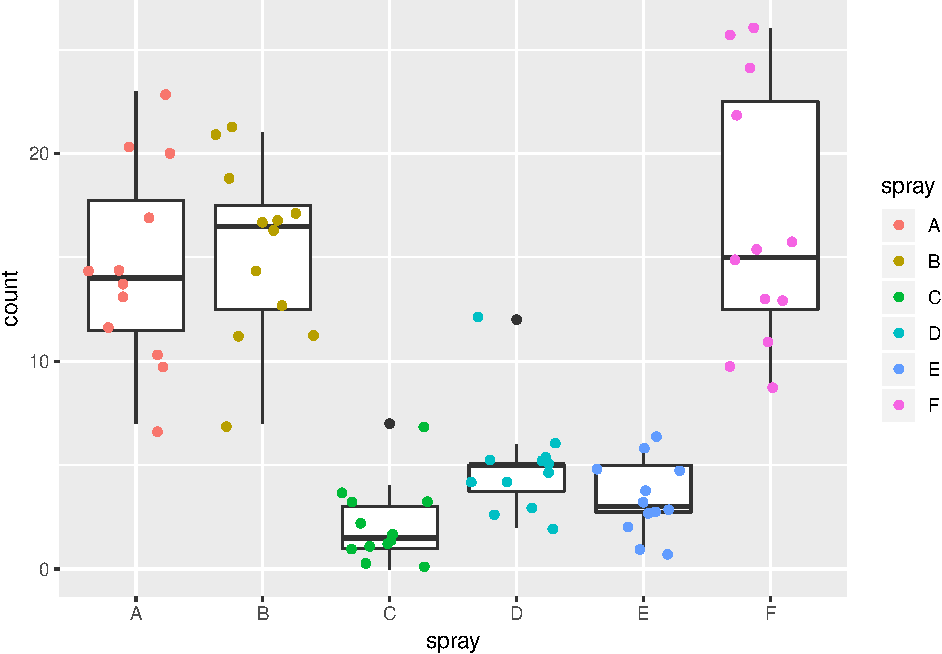
\includegraphics{AyduantiaStats_files/figure-latex/Visual-1.pdf}
\caption{\label{fig:Visual}Cuenta de insectos según tipo de insecticida}
\end{figure}

Para explorar visualmente si existe homogeneidad de varianza, se compraran las cajas y bigotes de los boxplots y se espera que tengan (Mas o menos distintos tamaños).

\hypertarget{test-de-bartlett}{%
\subsubsection{Test de Bartlett}\label{test-de-bartlett}}

Para realizar un test de homogeneidad de varianza se realiza el test de bartlett \citep{bartlett1937properties}, en este se usa nuestra conocida formula \emph{y \textasciitilde{} x}, esto es, y explicado por x junto a la función \emph{bartlett.test}. Para nuestro caso usaríamos:

\begin{verbatim}
## 
##  Bartlett test of homogeneity of variances
## 
## data:  count by spray
## Bartlett's K-squared = 25.96, df = 5, p-value = 9.085e-05
\end{verbatim}

Como en este caso, no el valor de p es menor a 0.05, decimos que no hay homogeneidad de varianza, por lo que no podemos hacer el test.

\hypertarget{normalidad-de-los-residuales}{%
\subsection{Normalidad de los residuales}\label{normalidad-de-los-residuales}}

En el caso de la base de datos \emph{iris}, demostraremos inmediatamente que si hay homogeneidad de varianza en el ancho del sépalo (Figura \ref{fig:IrisBox}):

\begin{figure}
\centering
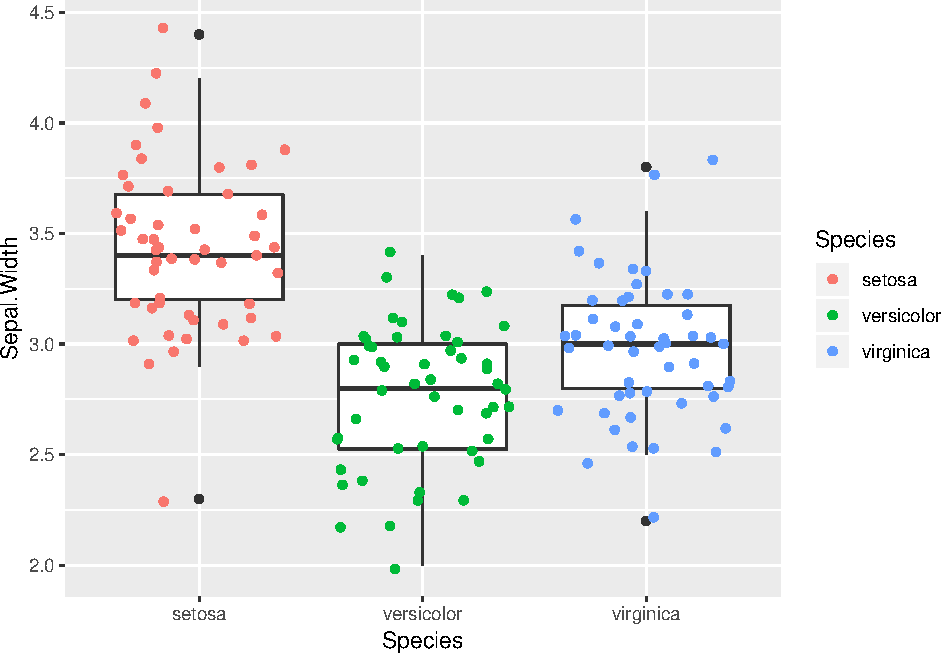
\includegraphics{AyduantiaStats_files/figure-latex/IrisBox-1.pdf}
\caption{\label{fig:IrisBox}Ancho de sépalo según especie del género Iris}
\end{figure}

\begin{verbatim}
## 
##  Bartlett test of homogeneity of variances
## 
## data:  Sepal.Width by Species
## Bartlett's K-squared = 2.0911, df = 2, p-value = 0.3515
\end{verbatim}

Debido a ello, podemos testar si los residuales tienen una distribución normalidad de los residuales, para esto lo primero que debemos hacer es un ANOVA, como fue explicado en el práctico anterior y guardar este objeto con un nombre:

\hypertarget{extraccion-de-los-residuales-del-modelo}{%
\subsubsection{Extracción de los residuales del modelo}\label{extraccion-de-los-residuales-del-modelo}}

Para extraer los residuales, podemos hacerlo de dos formas, si solo queremos un vector de sus valores, podemos extraerlo desde el modelo mismo utilizando \emph{\$residuals}. Si queremos guardarlo en un dataframe mas completo podemos utilizar la función \emph{augment} del paquete \emph{broom}.

La segunda opción nos entregará más información que podremos utilizar más tarde, pero ambas sirven para testear normalidad, la siguiente tabla muestra las primeras 6 observaciones generadas por la función \emph{augment}, donde \emph{resid}, son los residuales (Ver tabla \ref{tab:TabResid}.

\begin{table}

\caption{\label{tab:TabResid}primeras 6 observaciones del dataframe resultante de augment}
\centering
\begin{tabular}[t]{r|l|r|r|r|r|r|r|r}
\hline
Sepal.Width & Species & .fitted & .se.fit & .resid & .hat & .sigma & .cooksd & .std.resid\\
\hline
3.5 & setosa & 3.428 & 0.048 & 0.072 & 0.02 & 0.341 & 0.000 & 0.214\\
\hline
3.0 & setosa & 3.428 & 0.048 & -0.428 & 0.02 & 0.339 & 0.011 & -1.273\\
\hline
3.2 & setosa & 3.428 & 0.048 & -0.228 & 0.02 & 0.340 & 0.003 & -0.678\\
\hline
3.1 & setosa & 3.428 & 0.048 & -0.328 & 0.02 & 0.340 & 0.006 & -0.975\\
\hline
3.6 & setosa & 3.428 & 0.048 & 0.172 & 0.02 & 0.341 & 0.002 & 0.511\\
\hline
3.9 & setosa & 3.428 & 0.048 & 0.472 & 0.02 & 0.339 & 0.013 & 1.404\\
\hline
\end{tabular}
\end{table}

\hypertarget{inspeccion-visual-de-los-residuales}{%
\subsubsection{Inspección visual de los residuales}\label{inspeccion-visual-de-los-residuales}}

Existen dos formas de visualizar los residuales para determinar si la distribución de estos es o no es normal, histogramas y el qqplot.

\hypertarget{histograma}{%
\paragraph{Histograma}\label{histograma}}

Los histogramas nos darán una representación visual para tratar de entender si la distribución es normal, para esto, solo necesitamos usar el comando \emph{hist}, seguido del vector de los residuales, este es el comando para hacer el histograma (Figura \ref{fig:histogram}) con cualquiera de las dos bases de datos, el resultado debiera ser el mismo:

\begin{Shaded}
\begin{Highlighting}[]
\KeywordTok{hist}\NormalTok{(Residuales)}
\KeywordTok{hist}\NormalTok{(Resultados}\OperatorTok{$}\NormalTok{.resid)}
\end{Highlighting}
\end{Shaded}

\begin{figure}
\centering
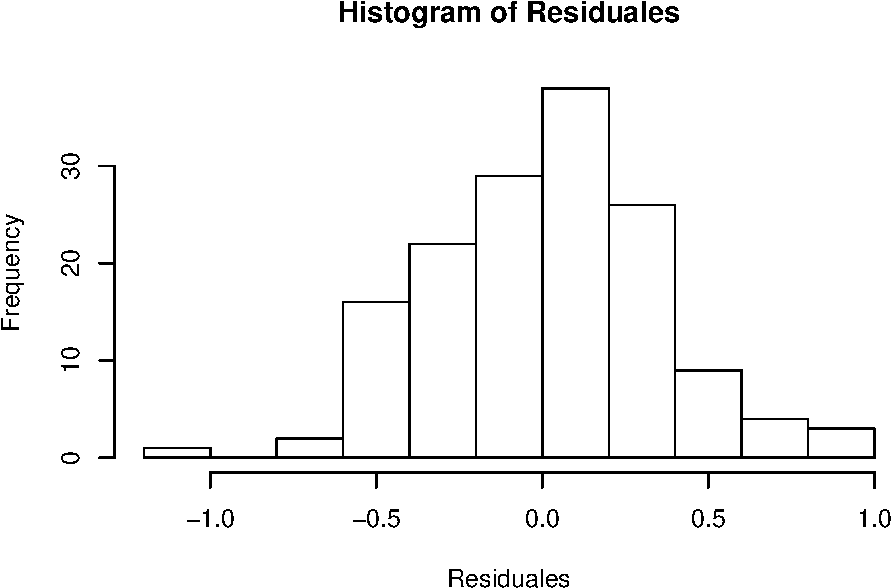
\includegraphics{AyduantiaStats_files/figure-latex/histogram-1.pdf}
\caption{\label{fig:histogram}Histograma de los resiudales del modelo ANOVA}
\end{figure}

\hypertarget{qqplot}{%
\paragraph{QQplot}\label{qqplot}}

El qq plot es otra forma visual de establecer si los residuales son o no son normales, para esto, lo esperado es que la gráfica resultante sea una diagonal lo mas recta posible, para esto usaremos la función \emph{qqnorm}, con nuestros residuales, de nuevo, podemos usar cualquiera de las dos versiones de nuestros datos:

\begin{Shaded}
\begin{Highlighting}[]
\KeywordTok{qqnorm}\NormalTok{(Residuales)}
\KeywordTok{qqnorm}\NormalTok{(Resultados}\OperatorTok{$}\NormalTok{.resid)}
\end{Highlighting}
\end{Shaded}

\begin{figure}
\centering
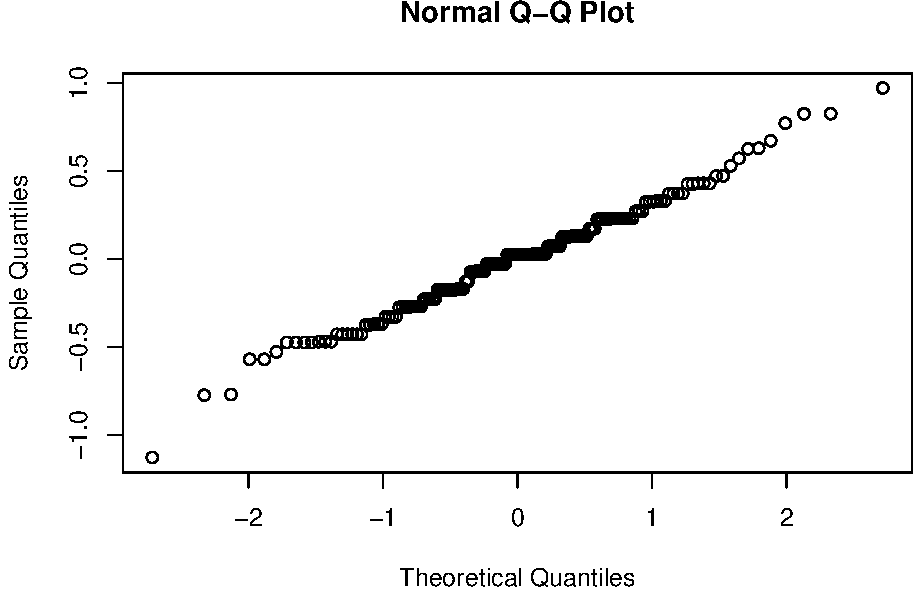
\includegraphics{AyduantiaStats_files/figure-latex/unnamed-chunk-19-1.pdf}
\caption{\label{fig:unnamed-chunk-19}qqplot de los resiudales del modelo ANOVA}
\end{figure}

\hypertarget{test-de-shapiro-para-determinar-normalidad}{%
\subsubsection{Test de Shapiro para determinar normalidad}\label{test-de-shapiro-para-determinar-normalidad}}

La forma más sencilla de determinar normalidad es usando el test de Shapiro-Wilk de normalidad \citep{royston1995remark}. Al igual que el test de Bartlett, si el valor de p es menor a 0.05, determinamos que la distribución de los datos no son normales, la función en \emph{R} para este test es \emph{shapiro.test}, y al igual que en los casos anteriores de \emph{hist} y \emph{qqpot}, solo necesitamos de usar un vector de residuales para ver el resultado del test. En nuestro caso:

\begin{Shaded}
\begin{Highlighting}[]
\KeywordTok{shapiro.test}\NormalTok{(Residuales)}
\KeywordTok{shapiro.test}\NormalTok{(Resultados}\OperatorTok{$}\NormalTok{.resid)}
\end{Highlighting}
\end{Shaded}

\begin{verbatim}
## 
##  Shapiro-Wilk normality test
## 
## data:  Residuales
## W = 0.98948, p-value = 0.323
\end{verbatim}

Ya que el valor de p es menor a 0.05, podemos decir que la distribución de nuestros residuales es normal, y por lo tanto el test cumple con los supuestos, y esto hace que sea valido el ANOVA, por lo que podemos ver nuestros resultados. La homogeneidad de Varianza es mas importante que la normalidad de residuales para estos casos, para ejemplos de lo que se debe hacer si se viola la normalidad ver \citet{lix1996consequences}

\hypertarget{actividad-2-suma-de-cuadrados}{%
\section{Actividad 2 Suma de cuadrados}\label{actividad-2-suma-de-cuadrados}}

Tanto los ANOVAS como las regresiones lineales se basan en minimizar la suma de cuadrados, es la suma de los cuadrados de los errores o residuales.

\hypertarget{que-es-el-error-por-que-al-cuadrado}{%
\subsection{¿Que es el error? ¿Por qué al cuadrado??}\label{que-es-el-error-por-que-al-cuadrado}}

\begin{figure}
\centering
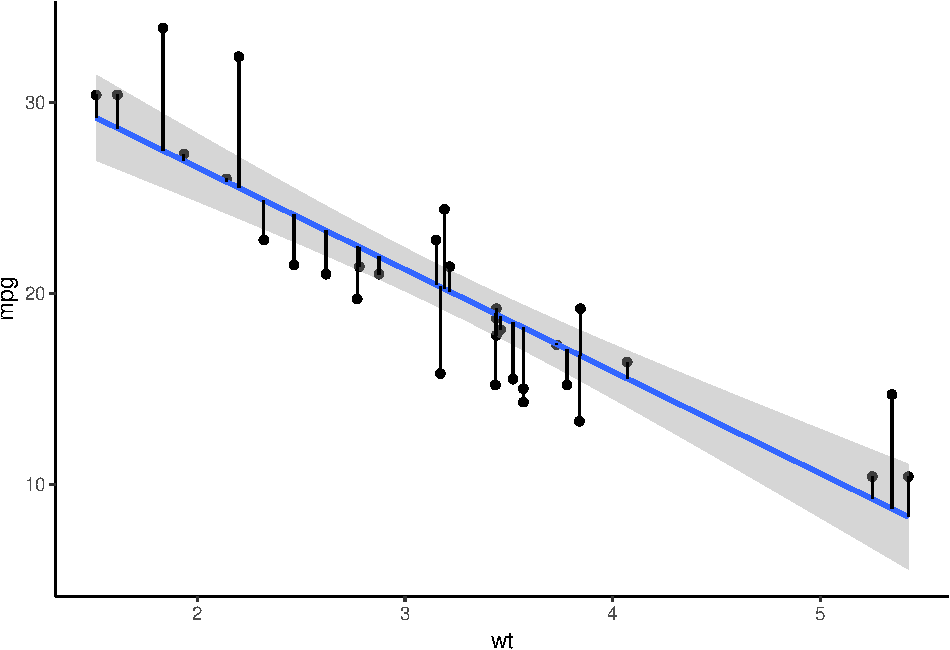
\includegraphics{AyduantiaStats_files/figure-latex/unnamed-chunk-22-1.pdf}
\caption{\label{fig:unnamed-chunk-22}Errores de una regresión lineal ejemplificados con la linea entre el valor predicho y el observado}
\end{figure}

En la figura y en la formula vemos ejemplificado que es el error, también conocido como residual, este es simplemente el valor observado

\[Observado - Predicho\]

El objetivo de todo modelo es el de minimizar estos errores, al ajustar el mejor modelo posible.

Los errores siempre se calculan al cuadrado, discutiremos por que en clase

\[\sum_{i=1}^{n} (Observado - Predicho)^2\]

\href{http://admin.derek-corcoran-barrios.com/shiny/rstudio/sample-apps/Shiny1/}{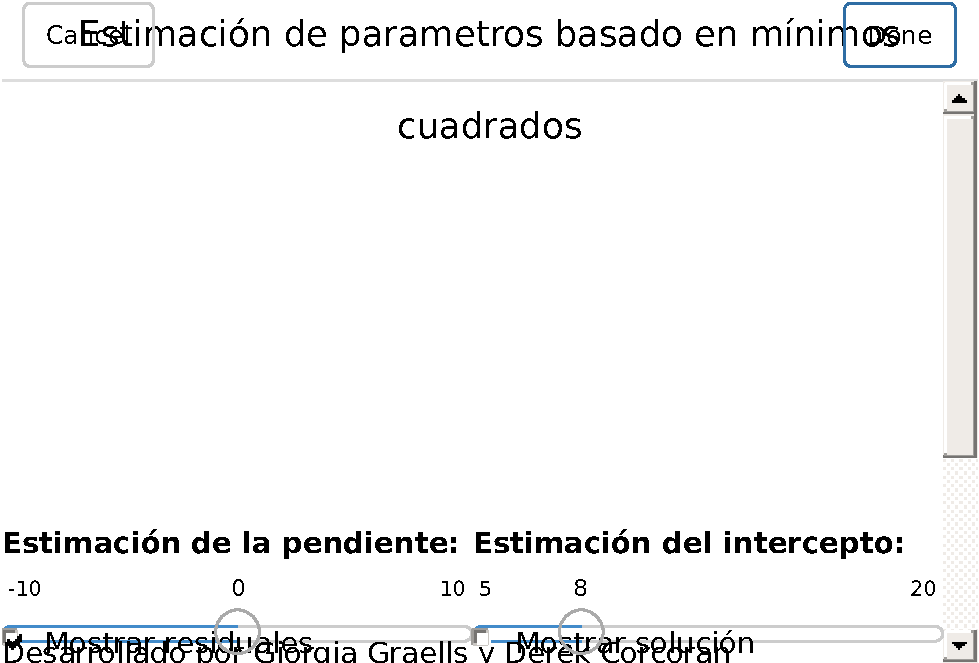
\includegraphics{AyduantiaStats_files/figure-latex/unnamed-chunk-23-1.pdf}}

\hypertarget{referencias}{%
\section{Referencias}\label{referencias}}

\hypertarget{Poder}{%
\chapter{Análisis de poder y primera tarea}\label{Poder}}

\hypertarget{obejtivos-del-practico}{%
\section{Obejtivos del práctico}\label{obejtivos-del-practico}}

\begin{itemize}
\tightlist
\item
  Entender cálculos de poder en base a matriz de confusión
\item
  Primera tarea de práctico
\end{itemize}

\hypertarget{matriz-de-confusion}{%
\section{Matriz de confusión}\label{matriz-de-confusion}}

La matriz de confusión es una herramienta de toma de decisiones, en el caso especial de la toma de decisiones tenemos la siguiente matriz de confusión (Tabla \ref{tab:errores})

\begin{table}

\caption{\label{tab:errores}Tabla de confusión de errores}
\centering
\begin{tabular}[t]{l|l|l}
\hline
  & Hipótesis nula cierta & Hipótesis alternativa cierta\\
\hline
Acepto hipótesis nula & No hay error & Error tipo 2\\
\hline
Acepto hipótesis alternativa & Error tipo 1 & No hay error\\
\hline
\end{tabular}
\end{table}

Esto puede ser fácilmente ejemplificado con el problema de una alarma de humo (tabla\ref{tab:Confucion}), en este caso cuando la alarma suena y no hay fuego y suena la alarma tenemos un error de tipo 1, en cambio si hay fuego y la alarma no suena tenemos un error de tipo 2

\begin{table}

\caption{\label{tab:Confucion}Matriz de confusión de una alarma de incendio}
\centering
\begin{tabular}[t]{lll}
\toprule
  & No hay fuego & Hay fuego\\
\midrule
No suena alarma & No hay error & Error tipo 2\\
Suena alarma & Error tipo 1 & No hay error\\
\bottomrule
\end{tabular}
\end{table}

\hypertarget{poder-y-matriz-de-confusion}{%
\subsection{Poder y matriz de confusión}\label{poder-y-matriz-de-confusion}}

\begin{itemize}
\tightlist
\item
  Probabilidad de que suene la alarma cuando no hay fuego

  \begin{itemize}
  \tightlist
  \item
    \(\alpha\) usualmente 5\%
  \item
    una de cada 20 alarmas es falsa
  \item
    ¿Cuál es el \(\alpha\) de una alarma de auto?
  \end{itemize}
\item
  Probabilidad de que no suene la alarma cuando hay fuego

  \begin{itemize}
  \tightlist
  \item
    \(\beta\) si es 10\% uno de cada 10 fuegos no es detectado
  \item
    poder es \(1-\beta\) confianza de que fuegos son detectados
  \end{itemize}
\end{itemize}

\hypertarget{calculo-de-poder-en-r}{%
\section{Calculo de poder en R}\label{calculo-de-poder-en-r}}

Para hacer cálculos de poder en ANOVAS de una y dos vías en \emph{R}, utilizamos el paquete \emph{pwr2} \citep{Pengcheng2017}. En este paquete podemos utilizar la función \emph{pwr.1way} para determinar el poder de un ANOVA de una vía, los argumentos de esta función son:

\begin{itemize}
\tightlist
\item
  \emph{K}: El número de grupos a testear
\item
  \emph{n}: Número de individuos por grupo
\item
  \emph{Alpha}: Nivel de significancia
\item
  \emph{Delta}: Valor mínimo a detectar
\item
  \emph{Sigma}: Desviación estándar de la muestra
\end{itemize}

Para cálculos precisos de n necesarios para muestras usar la siguiente app

\href{http://admin.derek-corcoran-barrios.com/shiny/rstudio/sample-apps/Shiny3/}{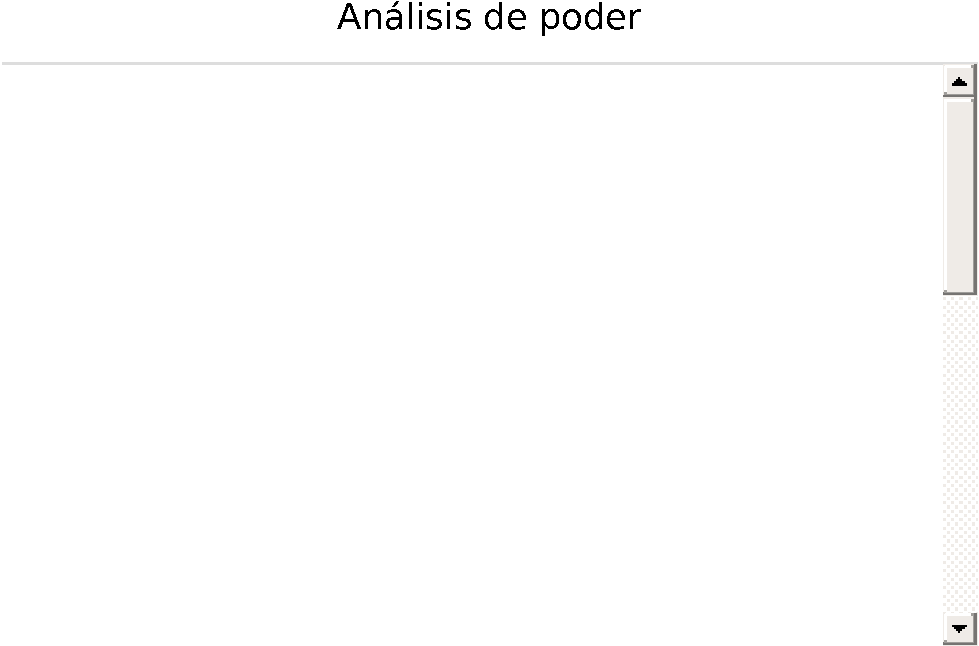
\includegraphics{AyduantiaStats_files/figure-latex/unnamed-chunk-27-1.pdf}}

\hypertarget{tarea}{%
\section{Tarea}\label{tarea}}

\hypertarget{el-problema}{%
\subsection{El problema}\label{el-problema}}

Una compañía que genera pesticidas descarga parte de sus desechos a un río. La ONG \textbf{RioSano}, dice que ha notado una alza en la mortalidad de los patos cortacorriente (\emph{Merganneta armata}) del río.

Ante esto la empresa contrata un científico, el cual hace una estimación de la mortalidad de patos en 10 zonas del río en que descargan sus desechos, y lo compara con otros dos ríos no contaminados. Este científico dice que no hay diferencias significativas en la mortalidad de los patos de los ríos con desechos y sin desechos con una confianza del 95\%. Para esto muestra como evidencia la figura 1 y tabla 3 e incluso hace públicos sus datos en el archivo \emph{MuestraPatos.csv}.

\begin{figure}
\centering
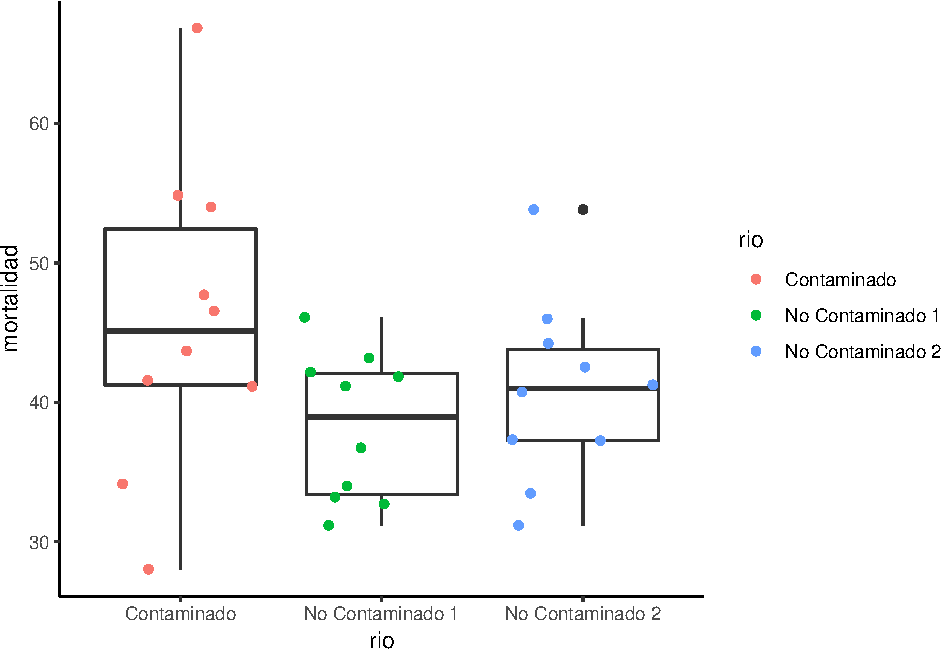
\includegraphics{AyduantiaStats_files/figure-latex/unnamed-chunk-28-1.pdf}
\caption{\label{fig:unnamed-chunk-28}Mortalidades calculadas en 10 zonas de tres ríos}
\end{figure}

\begin{table}

\caption{\label{tab:unnamed-chunk-29}Tabla de ANOVA de una vía de la mortalidad de patos de los tres ríos}
\centering
\begin{tabular}[t]{l|r|r|r|r|r}
\hline
term & df & sumsq & meansq & statistic & p.value\\
\hline
rio & 2 & 301.2531 & 150.62656 & 2.359899 & 0.1136188\\
\hline
Residuals & 27 & 1723.3436 & 63.82754 & NA & NA\\
\hline
\end{tabular}
\end{table}

La ONG \emph{RioSano} lo contrata para determinar la validez del estudio y si es necesario generar un estudio extra. Ante esto:

\begin{enumerate}
\def\labelenumi{\arabic{enumi}.}
\item
  Genere una matriz de confusión del problema y explique en este contexto que significaría el alfa y beta para este problema, y cual consideraría más relevante.
\item
  Diseñe el estudio que le gustaría hacer, determinando cuantas áreas debe muestrear por río, estime un delta mínimo que le gustaría determinar y el beta con el que se siente seguro y determine el \emph{n} mínimo necesario para ese estudio. Justifique su respuesta
\item
  Dado este \emph{n} mínimo realice lo siguiente

  \begin{itemize}
  \tightlist
  \item
    Realice un muestreo de n muestras por tipo de río del archivo \emph{Patos.csv}
  \item
    Genere gráficos y tablas exploratorias de los datos de su muestreo y describalas
  \item
    Revise los supuestos del ANOVA para su base de datos tanto gráficamente como con tests y determine si se puede realizar el anova
  \item
    Diga si según su diseño hay diferencias significativas en la mortalidad de patos entre los ríos
  \end{itemize}
\item
  Cada zona a muestrear requiere de un monitoreo exhaustivo, que tiene un costo de 500.000 pesos (esto es 1.500.000 de pesos si consideramos los 3 ríos). La ONG \emph{RioSano} consiguió 20.000.000 de pesos para este estudio. Dadas esas limitaciones, genere un balance de \(\alpha\), \(\beta\) y \(n\) dada esa limitación para hacer el mejor estudio posible dadas las consecuencias, justifique su respuesta.
\end{enumerate}

Genere un informe para la ONG \emph{RioSano} incorporando estos 5 puntos e incluya una introducción, metodología, resultados, discusión-conclusión y bibliografía, envíe el script de como generó los resultados

\hypertarget{t-student}{%
\chapter{Prueba t de Student}\label{t-student}}

Puedes encontrar una versión interactiva de esta guía \href{http://admin.derek-corcoran-barrios.com/shiny/rstudio/sample-apps/Interactivo5/}{aquí}.

La prueba t de student fue desarrollada por Gosset cuando trabajaba para la cervecería Guinness \citep{student1908probable}. Esta prueba permite comparar las medias de una muestra con la media teórica de una población, o comparar dos poblaciones. Una de las características de la prueba de student, es que permite la alternativa de ver si dos medias son diferentes o, si uno busca más confianza determinar si una media es mayor, o menor que otra. Para la prueba t de Student, se determina un valor de t, usando la siguiente formula (ecuación \eqref{eq:tStud}):

\begin{equation} 
  t = \frac{(\bar{x} - \mu)/(\frac{\sigma}{\sqrt{n}})}{s}
  \label{eq:tStud}
\end{equation}

El estadístico \(t\) posee un valor de p asociado dependiendo de los grados de libertad de la prueba.

\hypertarget{pruebas-de-una-muestra}{%
\subsection{Pruebas de una muestra}\label{pruebas-de-una-muestra}}

Las pruebas de una muestra nos permiten poner a prueba si la media de una población son distintas a una media teórica. Como ejemplo veremos el caso de las erupciones del géiser \emph{Old Faithful}, localizado en el Parque Nacional Yellowstone. Un guarda-parque del lugar dice que este géiser erupta cada 1 hora. Por suerte \emph{R} posee una base de datos de \citet{azzalini1990look} llamada \emph{faithfull}, la cual utilizaremos para determinar si esto es cierto o no usando la función \texttt{t.test}. Esta base de datos tiene dos columnas \emph{eruptions}, que muestra la duración en minutos de cada erupción y \emph{waiting} que presenta la espera en minutos entre erupciones.

Cuando usamos esta función con una muestra necesitamos llenar 2 argumentos:

\begin{itemize}
\tightlist
\item
  \textbf{x:} Un vector con los valores numéricos de a poner a prueba
\item
  \textbf{mu:} La media teórica a poner a prueba
\item
  \textbf{alternative:} Puede ser ``two.sided'', ``less'' o ``greater'', dependiendo de si uno quiere probar que la muestra posee una media distinta, menor o mayor que la media teórica.
\end{itemize}

En este caso haríamos lo siguiente

\begin{Shaded}
\begin{Highlighting}[]
\KeywordTok{data}\NormalTok{(}\StringTok{"faithful"}\NormalTok{)}
\KeywordTok{t.test}\NormalTok{(}\DataTypeTok{x =}\NormalTok{ faithful}\OperatorTok{$}\NormalTok{waiting, }\DataTypeTok{mu =} \DecValTok{60}\NormalTok{, }\DataTypeTok{alternative =} \StringTok{"two.sided"}\NormalTok{)}
\end{Highlighting}
\end{Shaded}

\begin{verbatim}
## 
##  One Sample t-test
## 
## data:  faithful$waiting
## t = 13.22, df = 271, p-value < 2.2e-16
## alternative hypothesis: true mean is not equal to 60
## 95 percent confidence interval:
##  69.27418 72.51994
## sample estimates:
## mean of x 
##  70.89706
\end{verbatim}

En este caso el valor de p nos dice que la media es diferente a 60.

\hypertarget{ejercicio-1}{%
\subsubsection{Ejercicio 1}\label{ejercicio-1}}

La base de datos \emph{airquality} (incorporada como ejemplo en \textbf{R}), muestra entre otras variables las partículas de ozono en Nueva York, cada día de Mayo a Septiembre de 1973 entre las 13:00 y las 15:00 \citep{chambers35graphical}. Supongamos que ustedes están a cargo de una agencia ambiental, y están estudiando en que meses deben reducir la actividad vehicular de Nueva York. Para esto planean disminuir a la mitad los pasajes del metro de Nueva York todos los meses que en promedio tengan sobre 55 ppb. Para esto deben comprobar estadisticamente que el mes en que harán esto tiene promedios sobre 55.

\hypertarget{pruebas-de-dos-muestras}{%
\subsection{Pruebas de dos muestras}\label{pruebas-de-dos-muestras}}

Las pruebas de dos muestras nos permiten ver si hay diferencias significativas entre las medias de dos muestras. En la base de datos \texttt{mtcars}, hay una columna que determina si los vehículos son de cambios manuales o automáticos. En este caso 0 significa automático y 1 significa manual. En la figura \ref{fig:autom} podemos ver una inspección gráfica de las posibles diferencias.

\begin{figure}
\centering
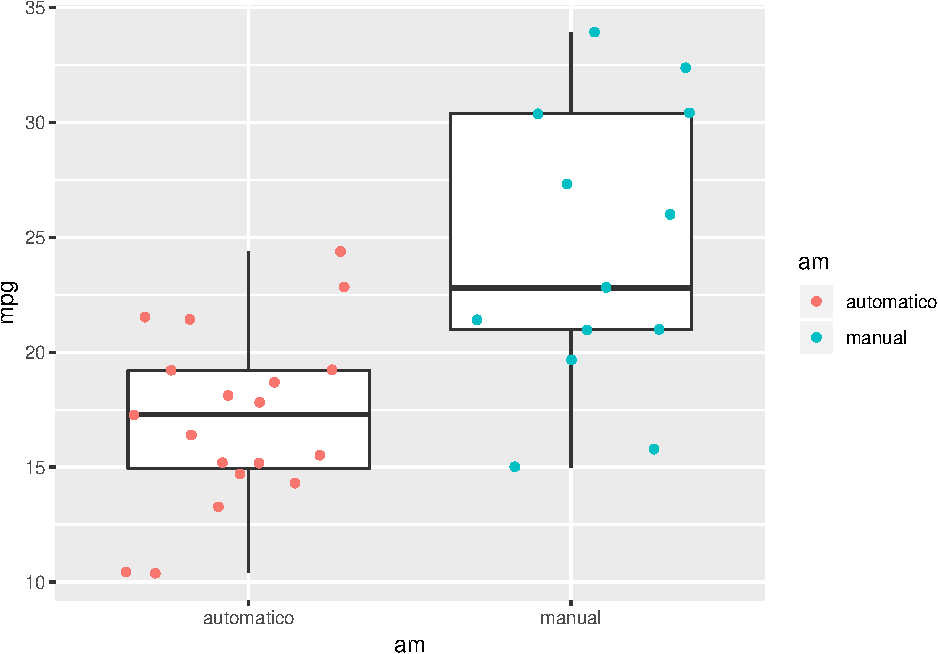
\includegraphics{AyduantiaStats_files/figure-latex/autom-1.pdf}
\caption{\label{fig:autom}Comparación de eficiencia entre vehiculos automaticos y manuales}
\end{figure}

Para hacer la comparación debemos agregar el argumento \texttt{var.equal} el cual en este caso asumiremos que es verdad, ya que en la próxima sección veremos los supuestos de la prueba t y las consecuencias de las violaciones de estos supuestos. En este caso podemos usar el símbolo \texttt{\textasciitilde{}} a ser leído como explicado por para la prueba t de dos muestras.

\begin{Shaded}
\begin{Highlighting}[]
\KeywordTok{t.test}\NormalTok{(mpg }\OperatorTok{~}\StringTok{ }\NormalTok{am, }\DataTypeTok{data =}\NormalTok{ mtcars, }\DataTypeTok{var.equal =}\OtherTok{TRUE}\NormalTok{)}
\end{Highlighting}
\end{Shaded}

\begin{verbatim}
## 
##  Two Sample t-test
## 
## data:  mpg by am
## t = -4.1061, df = 30, p-value = 0.000285
## alternative hypothesis: true difference in means is not equal to 0
## 95 percent confidence interval:
##  -10.84837  -3.64151
## sample estimates:
## mean in group 0 mean in group 1 
##        17.14737        24.39231
\end{verbatim}

En este caso se determinaría que los vehículos manuales (am = 1), son más eficientes que sus contra-partes automáticas.

\hypertarget{ejercicio-2}{%
\subsubsection{Ejercicio 2}\label{ejercicio-2}}

Para el siguiente ejercicio usaremos la base de datos \texttt{BeerDark} disponible en webcursos o en el siguiente \href{https://archive.org/download/BeerDark/BeerDark.csv}{link}. Esta base de datos posee 7 columnas, pero usaremos solo 4 de ellas:

\begin{itemize}
\tightlist
\item
  \textbf{Estilo:} Separa las cervezas entre Porters y Stouts
\item
  \textbf{Grado\_Alcoholico:} El grado alcohólico de las cervezas
\item
  \textbf{Amargor:} Valor IBU (International Bittering Units), a mayor valor más amarga la cerveza
\item
  \textbf{Color:} A mayor valor más oscura la cerveza.
\end{itemize}

Determinar si las cervezas Porter y Stouts son distintas en grado alcohólico, amargor y/o color.

\hypertarget{supuestos-de-la-prueba-de-t-y-alternativas}{%
\section{Supuestos de la prueba de t y alternativas}\label{supuestos-de-la-prueba-de-t-y-alternativas}}

Los supuestos de la t de student son las siguientes \citep{boneau1960effects}

\begin{itemize}
\tightlist
\item
  Independencia de las observaciones
\item
  Distribución normal de los datos en cada grupo
\item
  Homogeneidad de varianza
\end{itemize}

\hypertarget{prueba-de-una-muestra}{%
\subsection{Prueba de una muestra}\label{prueba-de-una-muestra}}

Como siempre la independencia de las muestras es algo que solo puede determinarse en base a el diseño del muestreo, y por otro lado, al haber solo una muestra, la homogeneidad de varianza no es un problema, en este caso solo podemos ver si la distribución es normal. Volviendo a nuestro ejemplo de una muestra, con la base de datos \texttt{faithfull}, veamos en base a un histograma (figura \ref{fig:Hist}), qqplot (figura \ref{fig:QQ}) y test de shapiro, si los datos son normales o no:

\begin{Shaded}
\begin{Highlighting}[]
\KeywordTok{hist}\NormalTok{(faithful}\OperatorTok{$}\NormalTok{waiting, }\DataTypeTok{xlab =} \StringTok{"Minutos de espera entre erupciones"}\NormalTok{)}
\end{Highlighting}
\end{Shaded}

\begin{figure}
\centering
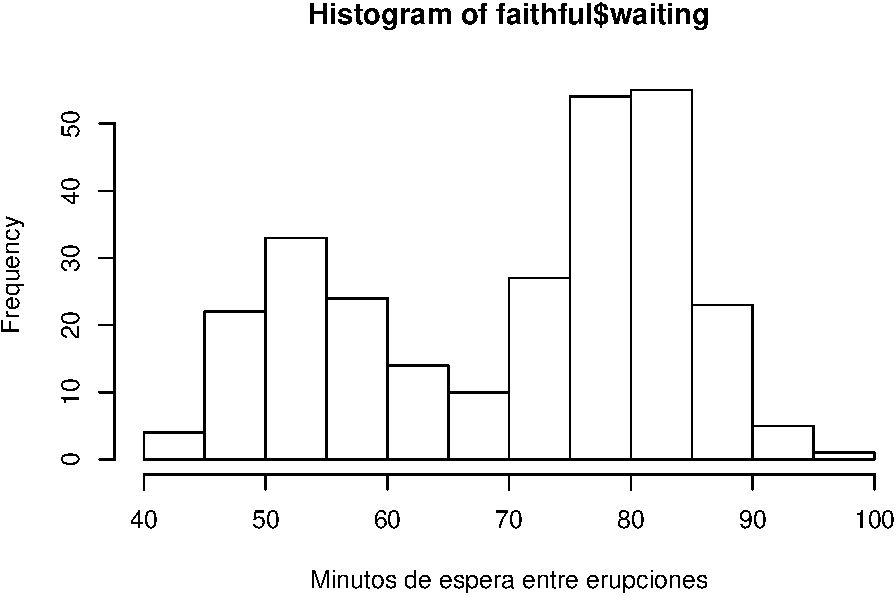
\includegraphics{AyduantiaStats_files/figure-latex/Hist-1.pdf}
\caption{\label{fig:Hist}Histograma de los minutos de espera de el géiser Old Fiathful}
\end{figure}

\begin{Shaded}
\begin{Highlighting}[]
\KeywordTok{qqnorm}\NormalTok{(faithful}\OperatorTok{$}\NormalTok{waiting)}
\end{Highlighting}
\end{Shaded}

\begin{figure}
\centering
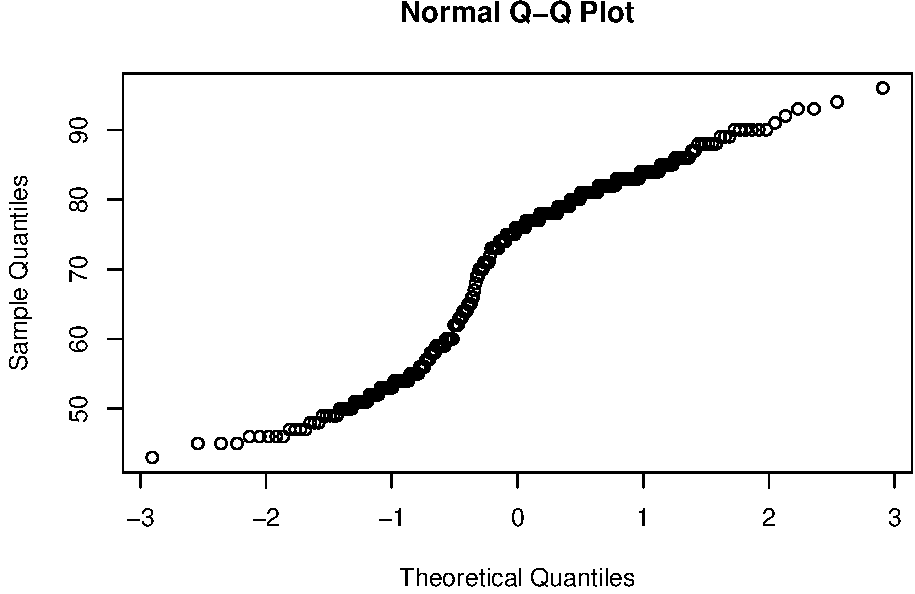
\includegraphics{AyduantiaStats_files/figure-latex/QQ-1.pdf}
\caption{\label{fig:QQ}QQplot de los minutos de espera de el géiser Old Fiathful}
\end{figure}

\begin{Shaded}
\begin{Highlighting}[]
\KeywordTok{shapiro.test}\NormalTok{(faithful}\OperatorTok{$}\NormalTok{waiting)}
\end{Highlighting}
\end{Shaded}

\begin{verbatim}
## 
##  Shapiro-Wilk normality test
## 
## data:  faithful$waiting
## W = 0.92215, p-value = 1.015e-10
\end{verbatim}

Como vemos en la figura 2, los datos no se ven normales, incluso se ven bimodales, lo cual significa que tiene 2 picos, en este caso uno al rededor de los 52 minutos y otro al rededor de los 85 minutos de espera (recordemos que la función \texttt{hist}, automáticamente usa el algoritmo de \citet{sturges1926choice}, para determinar como dividir los datos y obtener el mejor histograma). Nuestras sospechas de no normalidad son confirmadas al ver el qqplot, que no sigue para nada la diagonal, y es reafirmado por el test de shapiro, cuyo valor mucho menor a 0.05, nos dice que la distribución no es normal. Dado esto, debemos apelar a un test de distribución libre como el de \emph{Mann-Whitney}, la cual se realiza con la función \texttt{wilcox.test}, de la misma forma que es utilizada la función \texttt{t.test}, por lo tanto para nuestro ejemplo usamos:

\begin{Shaded}
\begin{Highlighting}[]
\KeywordTok{data}\NormalTok{(}\StringTok{"faithful"}\NormalTok{)}
\KeywordTok{wilcox.test}\NormalTok{(}\DataTypeTok{x =}\NormalTok{ faithful}\OperatorTok{$}\NormalTok{waiting, }\DataTypeTok{mu =} \DecValTok{60}\NormalTok{, }\DataTypeTok{alternative =} \StringTok{"two.sided"}\NormalTok{)}
\end{Highlighting}
\end{Shaded}

\begin{verbatim}
## 
##  Wilcoxon signed rank test with continuity correction
## 
## data:  faithful$waiting
## V = 31048, p-value < 2.2e-16
## alternative hypothesis: true location is not equal to 60
\end{verbatim}

Que en este caso nos lleva a la misma conclusión que nuestro ejemplo anterior.

\hypertarget{prueba-de-dos-muestras}{%
\subsection{Prueba de dos muestras}\label{prueba-de-dos-muestras}}

Para una prueba de dos muestras, podemos testear tanto la homogeneidad de varianza como la normalidad, para ver las dos cosas al mismo tiempo podemos usar un gráfico de violín (figura \ref{fig:Violin}). En este caso, las distribuciones no se ven muy diferentes a la normalidad, pero las varianzas se ven un tanto distintas, podemos seguir explorando esto visualmente usando la función \texttt{hist} previamente generando dos data frames, uno para autos automático y otro para manuales.

\begin{Shaded}
\begin{Highlighting}[]
\KeywordTok{data}\NormalTok{(}\StringTok{"mtcars"}\NormalTok{)}
\NormalTok{mt <-}\StringTok{ }\NormalTok{mtcars}
\NormalTok{mt}\OperatorTok{$}\NormalTok{am <-}\StringTok{ }\KeywordTok{ifelse}\NormalTok{(mtcars}\OperatorTok{$}\NormalTok{am  }\OperatorTok{==}\StringTok{ }\DecValTok{0}\NormalTok{, }\StringTok{"automatico"}\NormalTok{, }\StringTok{"manual"}\NormalTok{)}
\NormalTok{mt <-}\StringTok{ }\KeywordTok{as.data.frame}\NormalTok{(mt)}
\end{Highlighting}
\end{Shaded}

\begin{Shaded}
\begin{Highlighting}[]
\KeywordTok{ggplot}\NormalTok{(mt, }\KeywordTok{aes}\NormalTok{(}\DataTypeTok{x =}\NormalTok{ am, }\DataTypeTok{y =}\NormalTok{ mpg)) }\OperatorTok{+}\StringTok{ }\KeywordTok{geom_violin}\NormalTok{()}
\end{Highlighting}
\end{Shaded}

\begin{figure}
\centering
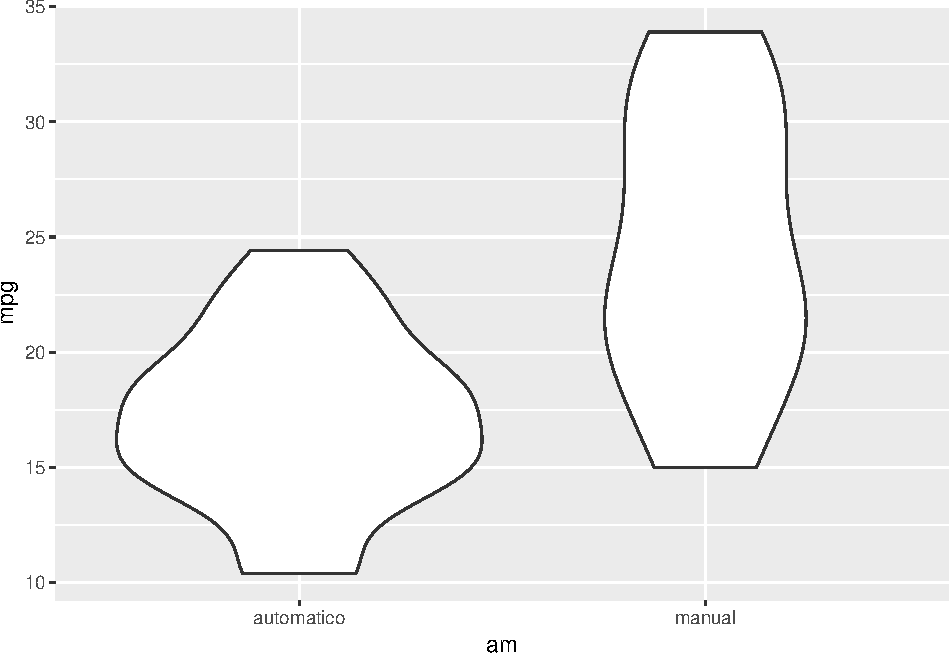
\includegraphics{AyduantiaStats_files/figure-latex/Violin-1.pdf}
\caption{\label{fig:Violin}Comparación de distribuciones y varianzas de los vehiculos automáticos}
\end{figure}

En este caso, las distribuciones no se ven muy diferentes a la normalidad, pero las varianzas se ven un tanto distintas, podemos seguir explorando esto separando los datos en vehículos automáticos y manuales para hacer histogramas, en este caso es importante que los ejes sean iguales, para eso en el histograma usaremos los parámetros ylim y xlim.

\begin{Shaded}
\begin{Highlighting}[]
\KeywordTok{hist}\NormalTok{(manuales}\OperatorTok{$}\NormalTok{mpg, }\DataTypeTok{xlim =} \KeywordTok{c}\NormalTok{(}\DecValTok{10}\NormalTok{,}\DecValTok{35}\NormalTok{), }\DataTypeTok{ylim =} \KeywordTok{c}\NormalTok{(}\DecValTok{0}\NormalTok{,}\DecValTok{5}\NormalTok{))}
\end{Highlighting}
\end{Shaded}

\begin{figure}
\centering
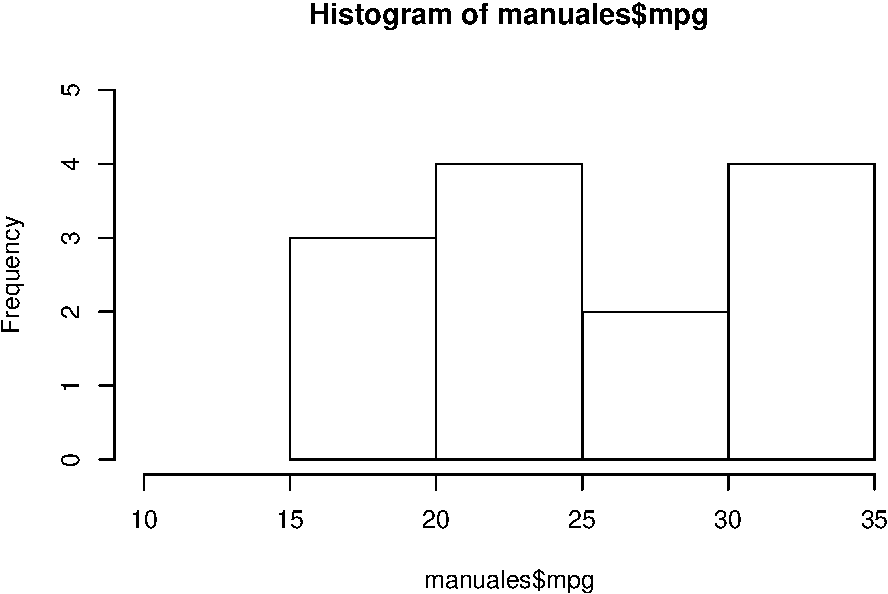
\includegraphics{AyduantiaStats_files/figure-latex/Manual-1.pdf}
\caption{\label{fig:Manual}Histograma de vehiculos manuales}
\end{figure}

\begin{Shaded}
\begin{Highlighting}[]
\KeywordTok{hist}\NormalTok{(autos}\OperatorTok{$}\NormalTok{mpg, }\DataTypeTok{xlim =} \KeywordTok{c}\NormalTok{(}\DecValTok{10}\NormalTok{,}\DecValTok{35}\NormalTok{), }\DataTypeTok{ylim =} \KeywordTok{c}\NormalTok{(}\DecValTok{0}\NormalTok{,}\DecValTok{5}\NormalTok{))}
\end{Highlighting}
\end{Shaded}

\begin{figure}
\centering
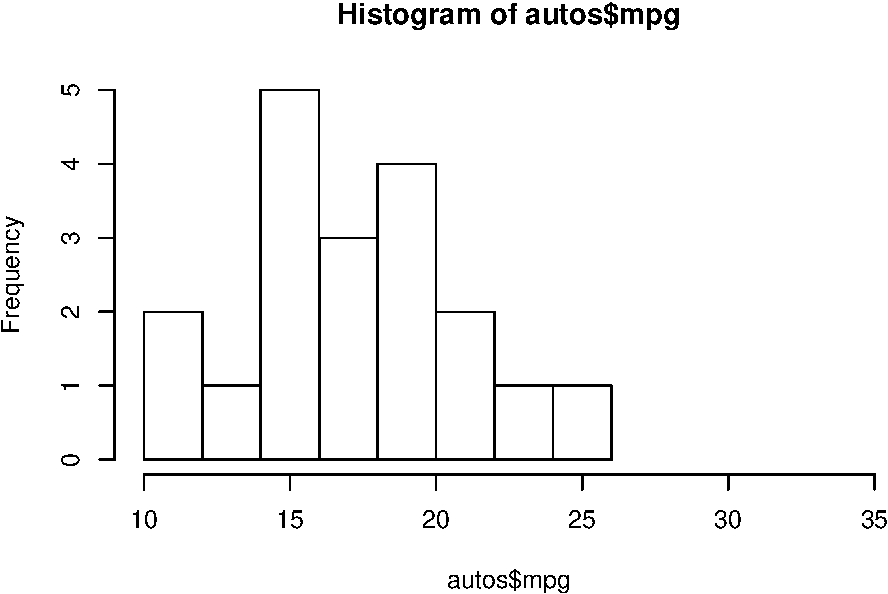
\includegraphics{AyduantiaStats_files/figure-latex/Auto-1.pdf}
\caption{\label{fig:Auto}Histograma de vehiculos automáticos}
\end{figure}

Como vemos, los vehículos manuales no parecen tener distribución normal como se ve en la figura \ref{fig:Manual}, esto podemos comprobarlo con el qqlot de los mismos datos (figura \ref{fig:qqManual})

\begin{Shaded}
\begin{Highlighting}[]
\KeywordTok{qqnorm}\NormalTok{(manuales}\OperatorTok{$}\NormalTok{mpg)}
\end{Highlighting}
\end{Shaded}

\begin{figure}
\centering
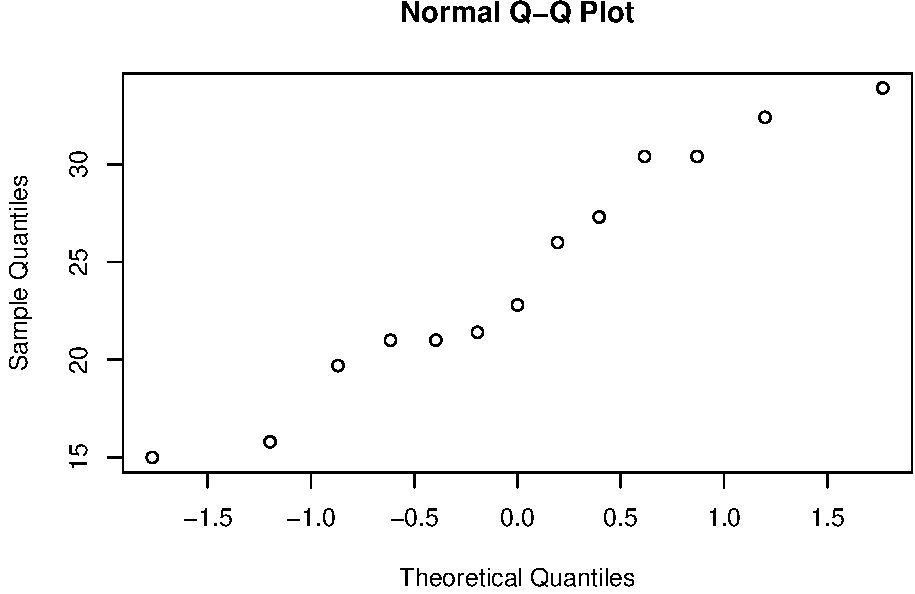
\includegraphics{AyduantiaStats_files/figure-latex/qqManual-1.pdf}
\caption{\label{fig:qqManual}QQplot de eficiencia de vehiculos con cambios manuales}
\end{figure}

\hypertarget{ejercicio-3}{%
\subsubsection{Ejercicio 3}\label{ejercicio-3}}

Como siempre la independencia de las muestras es algo que solo puede determinarse en base a el diseño del muestreo, y por otro lado, al haber solo una muestra, la homogeneidad de varianza no es un problema, en este caso solo podemos ver si la distribución es normal. Volviendo a nuestro ejercicio de una muestra, con la base de datos \texttt{airquality}, evalúe basado en histograma, qqplot y test de shapiro si se debe revaluar la hipótesis para los meses de julio y agosto

Para una prueba de dos muestras, podemos testear tanto la homogeneidad de varianza como la normalidad, para ver las dos cosas al mismo tiempo podemos usar un gráfico de violín \texttt{geom\_violin} en \emph{ggplot2}, lo cual puede seguir siendo explorando esto visualmente usando la función \texttt{hist} generando dos data frames, uno por cada clase de datos.

Evalúe si es necesario revaluar la hipótesis de que el amargor es distinto entre ambos estilos de cerveza

\hypertarget{bibliografia}{%
\section{Bibliografía}\label{bibliografia}}

\bibliography{book.bib}


\end{document}
